\renewcommand{\slideid}{L3-PY08}
\begin{frame}[c]{Python lab 4: replace the strong residual by energy}
\small
For the same Poisson problem and hard Dirichlet ansatz,
\[
 \Energy(u_\theta)=\int_0^1\left[\tfrac12(u_\theta')^2
           -\pi^2\sin(\pi x)u_\theta\right]\dd x.
\]
\lstinputlisting[style=pythonlab]{experiments/snippets/ritz_loss.py}
\begin{block}{First derivatives suffice}
Use Gauss--Legendre nodes and weights on $[0,1]$.
The same network initialization isolates the change of objective.
\end{block}
\labnote{\RitzProtocol.}
\end{frame}

\renewcommand{\slideid}{L3-PY09}
\begin{frame}[c]{Python output: compare errors, not raw loss values}
\small
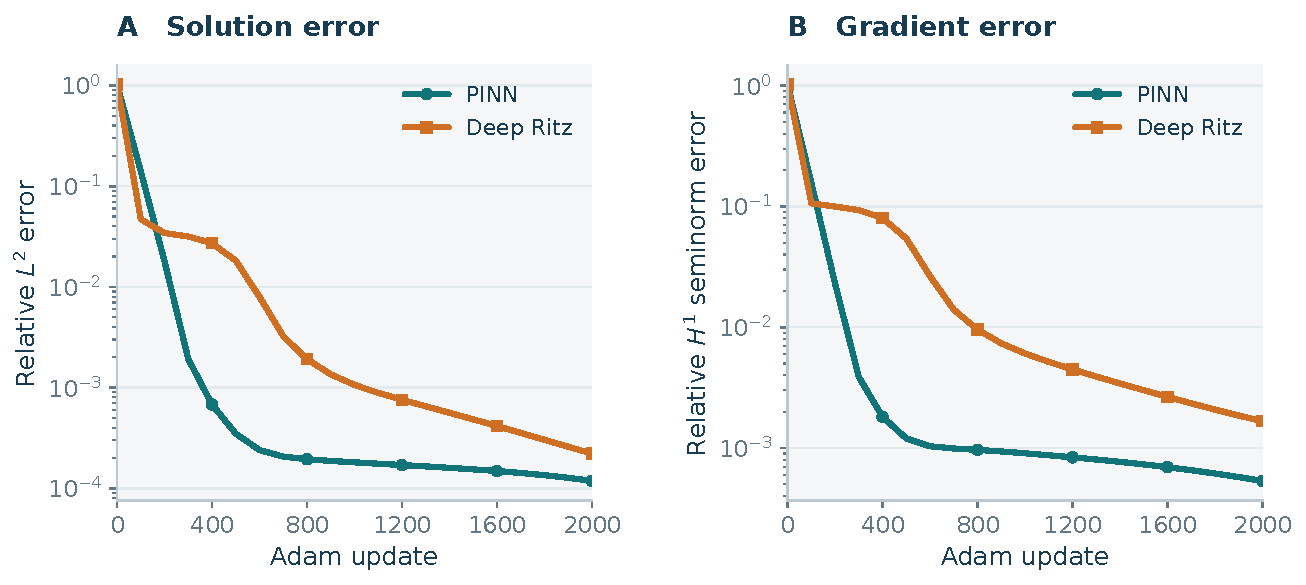
\includegraphics[width=\textwidth]{experiments/figures/ritz_comparison.pdf}
\begin{block}{Final evaluation after optimizer refinement}
\begin{tabular}{@{}lcc@{}}
 & relative $L^2$ error & relative $H^1$ seminorm error\\
PINN & \ForwardLtwo & \ForwardHone\\
Deep Ritz & \RitzLtwo & \RitzHone
\end{tabular}
\end{block}
\labnote{Curves show Adam only; the table includes subsequent L-BFGS refinement.
Equal updates do not imply equal runtime. One seed, one smooth problem.}
\end{frame}
\renewcommand{\slideid}{L3}
